% !TeX encoding = UTF-8
% !TeX spellcheck = pl_PL

% $Id:$
%% Konfiguracja:
\newcommand{\formakursu}{Projekt}
\newcommand{\kurs}{Teoria i metody optymalizacji}
\newcommand{\doctype}{Harmony Search}
\newcommand{\osobaA}{Artur \textsc{Gasi\'nski}, 218685}
\newcommand{\osobaB}{Bartosz \textsc{Lenartowicz}, 218518}
\newcommand{\termin}{wt 9:15-11:00}

\newcommand{\prowadzacy}{Dr in\.{z}. Ewa \textsc{Szlachcic}}
\documentclass[10pt, a4paper]{article}
\usepackage{listings}

%Preambuła dokumentu

% linki w spisie tresci, bibliografi
\usepackage[bookmarks=true,bookmarksnumbered=false,unicode=true,pdftex=true, colorlinks,filecolor=black,linkcolor=black,urlcolor=black,citecolor=black]{hyperref}

%ustawienie rozmiaru papieru
\usepackage[a4paper, left=2.5cm, right=2.5cm, top=2.5cm, bottom=2.5cm, headsep=1.2cm]{geometry}

%rozmaite ustawienia pozwalające okreslić język

%NALEŻY wybrać jeden z pakietów
%\usepackage{polski} %przydatne podczas składania dokumentów w j. polskim
\usepackage[polish]{babel}  % pakiet lokalizujący dokument w języku polskim
%\usepackage[british]{babel}

\usepackage{indentfirst}	% polski styl pisania (np. rozpoczecie pierwszego akapitu
% pod nazwa rozdzialu od wciecia)
%\usepackage[OT4]{fontenc}
\usepackage[utf8]{inputenc} % w miejsce utf8 można wpisać latin2 bądź cp1250,
% w zależności od tego w jaki sposób kodowane są 
% polskie znaki diakrytyczne przy wprowadzaniu 
% z klawiatury.
%kodowanie znaków, zależne od systemu
\usepackage[T1]{fontenc} %poprawne składanie polskich czcionek

%OPEROWANIE NA OBRAZACH
\usepackage{graphicx}       % pakiet graficzny, umożliwiający m.in.
% import grafik w formacie eps
%\usepackage{epstopdf}		% pozwala na importowanie grafik w formacie eps
% przy użyciu pdflatex
\usepackage[update,prepend]{epstopdf}
\usepackage{rotating}       % pakiet umożliwiający obracanie rysunków
\usepackage{subfigure}      % pakiet umożliwiający tworzenie podrysunków
\usepackage{epic}           % pakiet umożliwiający rysowanie w środowisku latex
\usepackage{psfrag}         % pakiet umożliwiający podmianę łańcuchów znaków 
% w plikach eps
%\usepackage{curves}         % pakiet do wykreslania krzywych

%pakiety dodające dużo dodatkowych poleceń matematycznych
\usepackage{amsfonts}       % pakiet z rozmaitymi czcionkami matematycznymi
%\usepackage{amssymb}        % pakiet z rozmaitymi symbolami matematycznymi
\usepackage{amsmath}        % pakiet z rozmaitymi środowiskami matematycznymi

\usepackage{fp}             % pakiet z funkcjami operujacymi 
% na liczbach zmiennoprzecinkowych
\usepackage{calc}           % pakiet umożliwiający operacje arytmetyczne
% na tzw. licznikach (liczbach całkowitych)
\usepackage{leftidx}		% indeksy górne i dolne po lewej stronie

%definicje matematyczne
\providecommand{\abs}[1]{\lvert#1\rvert}
\providecommand{\norm}[1]{\lVert#1\rVert}

%pakiety wspomagające i poprawiające składanie tabel
\usepackage{supertabular}
\usepackage{array}
\usepackage{tabularx}
\usepackage{hhline}
\usepackage{longtable}		% wsparcie dla dlugich tabel
\usepackage{multicol}		% podzial strony na wiele kolumn

%pakiet do BibTex
\usepackage{cite}

\usepackage{url} %pakiet pozawalający na dodawanie adresów url w bibliografi

%pakiet wypisujący na marginesie etykiety równań i rysunków zdefiniowanych przez \label{}, chcąc wygenerować finalną wersję dokumentu wystarczy usunąć poniższą linię
%\usepackage{showlabels}

\usepackage{float}			% lepsza obsluga mechanizmow obiektow plywajacych
% wymuszenie wstawienia np. tabeli, obrazka w danym miejscu przez [H]

\usepackage{listings}       % pakiet dedykowany zrodlom programow
\usepackage{color}


\definecolor{dkgreen}{rgb}{0,0.6,0}
\definecolor{gray}{rgb}{0.5,0.5,0.5}
\definecolor{mauve}{rgb}{0.58,0,0.82}

\lstset{ %
	language=Matlab,                % the language of the code
	basicstyle=\scriptsize,           % the size of the fonts that are used for the code
	numbers=left,                   % where to put the line-numbers
	numberstyle=\tiny\color{gray},  % the style that is used for the line-numbers
	stepnumber=1,                   % the step between two line-numbers. If it's 1, each line 
	% will be numbered
	numbersep=5pt,                  % how far the line-numbers are from the code
	backgroundcolor=\color{white},      % choose the background color. You must add \usepackage{color}
	showspaces=false,               % show spaces adding particular underscores
	showstringspaces=false,         % underline spaces within strings
	showtabs=false,                 % show tabs within strings adding particular underscores
	%frame=single,                   % adds a frame around the code
	rulecolor=\color{black},        % if not set, the frame-color may be changed on line-breaks within not-black text (e.g. comments (green here))
	tabsize=2,                      % sets default tabsize to 2 spaces
	captionpos=b,                   % sets the caption-position to bottom
	breaklines=true,                % sets automatic line breaking
	breakatwhitespace=false,        % sets if automatic breaks should only happen at whitespace
	%title=\lstname,                   % show the filename of files included with \lstinputlisting;
	% also try caption instead of title
	keywordstyle=\color{blue},          % keyword style
	commentstyle=\color{dkgreen},       % comment style
	stringstyle=\color{mauve},         % string literal style
	escapeinside={\%*}{*)},            % if you want to add LaTeX within your code
	morekeywords={*,...},              % if you want to add more keywords to the set
	deletekeywords={...}              % if you want to delete keywords from the given language
}

%polish signs in lst code
\lstset{literate=%
	{ą}{{\k{a}}}1
	{ć}{{\'c}}1
	{ę}{{\k{e}}}1
	{ł}{{\l}}1
	{ń}{{\'n}}1
	{ó}{{\'o}}1
	{ś}{{\'s}}1
	{ż}{{\.z}}1
	{ź}{{\'z}}1
	{Ą}{{\k{A}}}1
	{Ć}{{\'C}}1
	{Ę}{{\k{E}}}1
	{Ł}{{\L}}1
	{Ń}{{\'N}}1
	{Ó}{{\'O}}1
	{Ś}{{\'S}}1
	{Ż}{{\.Z}}1
	{Ź}{{\'Z}}1
}

\usepackage{verbatim}       % pakiet dedykowany rozmaitym wydrukom tekstowym
\usepackage{ifthen}         % pakiet umożliwiający tworzenie prostych programów
% (m.in. zawiera instrukcje powtórzeniowe 
% i warunkowe)
\usepackage{upquote}		%normal quotations marks ' and `

% deklaracje wymagane przez pakiet theorem automatycznie ladowany w przypadku
% klasy dokumentu article
%
\newtheorem{Dn}{Definicja}[section]     % deklaracja srodowiska definicja
\newtheorem{La}[Dn]{Lemat}                % deklaracja srodowiska lemat
\newtheorem{Tm}[Dn]{Twierdzenie}          % deklaracja srodowiska twierdzenie
\newtheorem{Rk}[Dn]{Spostrze{\.z}enie}  % deklaracja srodowiska spostrzezenie
\newtheorem{Am}[Dn]{Algorytm}           % deklaracja srodowiska algorytm
\newtheorem{As}[Dn]{Za{\l}o{\.z}enie}   % deklaracja srodowiska zalozenie
\newtheorem{Pn}[Dn]{Propozycja}           % deklaracja srodowiska propozycja
\newtheorem{Py}[Dn]{W{\l}asno{\'s}{\'c}}  % deklaracja srodowiska wlasnosc
\newtheorem{Cy}[Dn]{Wniosek}              % deklaracja srodowiska wniosek
\newtheorem{Ee}[Dn]{Przyk{\l}ad}        % deklaracja srodowiska przyklad
\newtheorem{Ex}{{\'C}wiczenie}          % deklaracja srodowiska cwiczenie

%helps to specify width of a column in table
%\begin{tabular}{|C{1cm}|c|c|c|c|c|c|c|c|c|c|}
%first column will have widht of 1cm
\newcolumntype{L}[1]{>{\raggedright\let\newline\\\arraybackslash\hspace{0pt}}m{#1}}
\newcolumntype{C}[1]{>{\centering\let\newline\\\arraybackslash\hspace{0pt}}m{#1}}
\newcolumntype{R}[1]{>{\raggedleft\let\newline\\\arraybackslash\hspace{0pt}}m{#1}}

\sloppy			%zawija bardzo długie linie

%\pagenumbering{gobble}% Remove page numbers (and reset to 1)
\begin{document}
\def\tablename{Tabela}	%zmienienie nazwy tabel z Tablica na Tabela
\begin{titlepage}
	\begin{center}
		\textsc{\LARGE \formakursu}\\[1cm]		
		\textsc{\Large \kurs}\\[0.5cm]		
		\rule{\textwidth}{0.08cm}\\[1cm]
		{\huge \bfseries \doctype}\\[1cm]
		\rule{\textwidth}{0.08cm}\\[1cm]
		\begin{flushright} \large
		\emph{Autor: }\\
		\osobaA\\
		\osobaB\\[0.4cm]
		\emph{Termin: }\termin\\[0.4cm]
		\emph{Prowadzący:} \\
		\prowadzacy \\
		\end{flushright}
		\vfill
		{\large \today}
	\end{center}	
\end{titlepage}
\newpage
\tableofcontents
\newpage

\section{Sformułowanie zadania optymalizacji}
\label{sec:1}
Większość metod optymalizacji procesów produkcyjnych czy logistycznych sprowadza się do przedstawienia zależności pomiędzy procesami za pomocą okrelonej funkcji celu {\em f(x)}. Pod postacią zmiennych {\em x}~tego równania ukazane są parametry procesów, którymi można manipulować.  By właściwie zoptymalizować proces, należy znaleźć minimum bądź maksimum (najlepiej globalne) funkcji {\em f(x)=f*(x*)}. Obliczanie minimalnej bądź maksymalnej wartości {\em f*}, zależnej od wielu zmiennych {\em x} w pożądanym czasie jest problematyczne. Istnieją algorytmy specjalizujące się w  rozwiązywaniu zadań tego typu. Niniejsza praca została napisana by przedstawić jeden z nich -- Harmony Search. Został on przedstawiony w 2001 przez Zong Woo Geema, Joong Hoon Kima oraz G.V. Loganathana w pracy ,,A New Heuristic Optimization Algorithm: Harmony Search'' \cite{bib:orginal}.

\section{Szczegółowe omówienie algorytmu optymalizacji}
\label{sec:2}
Inspiracją dla algorytmu było szukanie przez muzyków jazzowych najlepszych harmonii dźwięków podczas improwizacji. Jego matematyczny odpowiednik umożliwia optymalizację funkcji {\em f(x)} wielu zmiennych. 

Algorytm do działania wymaga zainicjowania {\em $m=4+2*n$} wartości początkowych. Jedynym kryterium stopu algorytmu jest liczba iteracji $L$. Głównym elementem algorytmu jest pamięć harmonii {\tt HM} ({\em ang. harmony memory}). Jest to zbiór zapamiętanych rozwiązań funkcji $f(x)$ wraz z wartościami argumentów $x$, dla których została obliczona funkcja. Schemat tablicy {\tt HM} umieszczony jest na rysunku \ref{tab:1}. Wielkość pamięci {\em HMS} deklarowana jest z góry przez użytkownika i podczas kolejnych iteracji nie zmienia rozmiaru. Wymagane jest również by na początku działania określić przedział wartości $[a,b]$ dla każdej zmiennej $x_{1}=[a_{1},b_{1}], ... ,x_{n}=[a_{n},b_{n}]$, z którego będą wyszukiwane rozwiązania dlatego należy zadeklarować $2*n$ wartości gdzie $n$ jest ilością zmiennych równania. Dodatkowo wymagane jest określenie dwóch prawdopodobieństw. Pierwsze {\tt HMCR} ({\em ang. harmony memory consideration ratio}) określa współczynnik doboru tonu z pamięci, drugie {\tt PAR} ({\em ang. pitch adjustment ratio}) nazywane jest współczynnikiem dostosowania tonu. Oczywistym jest, że przedział wartości prawdopodobieństw określany jest na $<0,1>$.

Algorytm działa następująco: wpierw program wypełnia tablicę pamięci harmonii {\tt HM} początkowymi wartościami. Każda wartość $x$ losowana jest z swojego ograniczonego przedziału $[a,b]$. Gdy tablica zostanie zapełniona rozpoczyna się część iteracyjna algorytmu. Polega na wyszukiwaniu kolejnego rozwiązania poprzez wyznaczanie kolejnych rozwiązań wedle trzech reguł. Pierwsza mówi, że z prawdopodobieństwem $P_{1}={\tt HMCR}$ wartość nowej zmiennej $x_{n}$ wybierana jest z pośród zmiennych zapamiętanych w tablicy {\tt HM}. Druga, że wartością prawdopodobieństwa $P_{2}=(1-{\tt HMCR})$ wartość zmiennej losowana jest z całego przedziału $[a,b]$, a zasada trzecia, że zmienna ustalona w regule pierwszej modyfikowana jest z prawdopodobieństwem $P_{3}=({\tt HMCR}*{\tt PAR})$. W praktyce reguła trzecia sprowadza się do dodania do wylosowanej zmiennej $x$ z reguły pierwszej liczby z przedziału $<-c,c>$. Następnie gdy zostaną wylosowane wszystkie wartości $x_{n}$ obliczana jest dla nich wartość funkcji $f(x)$. Jest ona porównywana z wartościami umieszczonymi w tablicy {\tt HM}. Jeżeli jest mniejsza niż największa wartość z tablicy, zamienia się ją z największą wartością (najgorszym rozwiązaniem). Na tym kończy się iteracja. Następnie wykonuje się kolejne iteracje do osiągnięcia maksymalnej ilości iteracji {\em $L$}. Polski opis algorytmu można również znaleźć np. w~pracy \cite{bib:tlumaczenie}.
\begin{figure}[h]
\begin{tabular}{|ccc|c|}
	\hline 
	$x_{11}$ & $\cdots$ & $x_{n1}$ & $=f_{1}$\\ 
	\hline 
	$\vdots$ & $\ddots$ & $\vdots$ & $\vdots$\\ 
	\hline 
	$x_{1HMS}$ & $\cdots$ & $x_{nHMS}$ & $=f_{HMS}$\\ 
	\hline 
\end{tabular}
	\centering
	\caption{Schemat tabeli {\em Harmony Memory}}
	\label{tab:1}
\end{figure}

\pagebreak

\section{Informacje o programie}
\label{sec:implementacja}
Program do obliczania minimum funkcji na podstawie algorytmu Harmony Search został napisany w~języku Java. Technologią dostarczającą GUI dla użytkownika była {\em JavaFx} umożliwiająca tworzenie aplikacji okienkowych. Dodatkowo by ułatwić zarządzanie bibliotekami wewnątrz projektu użyto wsparcia ze strony {\em Maven}.  Program korzysta z zewnętrznej biblioteki mXparser do parsowania łańcuchów znakowych na funkcje i do obliczania ich wartości w określonych punktach \cite{bib:mathparser}. Wykres prezentujący najlepsze rozwiązanie zaznaczone na wykroju z przestrzeni rozwiązań funkcji został stworzony za pomocą biblioteki {\em jzy3D}.

\subsection{Środowisko programistyczne, zastosowane biblioteki i gotowe moduły}
\label{subsec:gui}
By ułatwić wprowadzanie funkcji do programu oraz bezproblemowo odczytywać wyniki obliczone przez program zostało stworzone GUI programu. Na rysunkach \ref{fig:1}, \ref{fig:2} i \ref{fig:3} przedstawiono etapy działania programu. Poszczególne elementy GUI podczas działania programu nie zmieniają swojego położenia. Jedynie pustych w miejscach zostają wyświetlone ich parametry, dlatego by omówić elementy posłużono się rysunkiem \ref{fig:3}, gdzie widnieje obraz programu po obliczeniach. Główne okno programu zostało podzielone pionowo na trzy części. Pierwsza część od lewej przeznaczona jest do wpisania funkcji i jej parametrów, środkowa prezentuje wykres, a część prawa w tabelce wyniki obliczeń programu. Wszystkie części zostaną szczegółowo opisane poniżej.

\subsection{Parametry}
\label{subsec:parametry}
W części parametrów można dostrzec, że zaraz pod paskiem edycji znajduje miejsce do wpisania funkcji, której minimum należy wyznaczyć. Okno umożliwia również wybór takiej funkcji z wcześniej zadeklarowanych w programie. Dokonuje się tego, klikając w rozwijane menu. Zostało to przedstawione na rysunku \ref{fig:1}. Po wybraniu funkcji automatycznie zostaną domyślnie uzupełnione wszystkie parametry obliczeń. Oczywiście możliwa jest dostosowanie algorytmu do własnych potrzeb. Poniżej okna funkcji znajduje się przycisk ,,{\tt Resetuj wartości parametrów}'' umożliwiający, jak mówi nazwa przywrócenie domyślnych wartości parametrów. Poniżej przycisku zostały umieszczone po sobie cztery główne parametry algorytmu {\em Harmony Search}. 

Pierwszy z parametrów {\tt HMS} ({\em ang. harmony memory size}) reguluje ilość zapamiętywanych rozwiązań podczas wyszukiwania. Domyślnie rozmiar jest zadeklarowany na $20$. Poniżej znajduje się okno o nazwie {\tt iteracje}. Domyślnie jest zadeklarowana maksymalna wartość iteracji równa $10000$. W każdej iteracji programu algorytm wyszukuje nowe rozwiązanie i sprawdza je z~tymi zapisanymi w {\tt HMS}. Im większa liczba iteracji, tym algorytm powinien obliczać dokładniejsze rozwiązanie, kosztem wydłużonego czasu obliczeń. Następnie pod polem {\tt iteracje} znajduje się pole {\tt HMCR} ({\em ang. harmony memory consideration ratio}). Jest to prawdopodobieństwo wyboru rozwiązania z pamięci (z zakresu $(0, 1)$). Im {\tt HMCR} jest większe tym wyszukiwane wartości {\em x} następnych rozwiązań będą zbliżone do tych istniejących już w tablicy {\tt HMS}. Poniżej znajduje się drugi parametr prawdopodobieństwa o nazwie {\tt PAR} {\em(ang. pitch adjustment ratio)} tłumaczony jako współczynnik dostosowywania tonu. Wybierany jest również z zakresu $(0, 1]$. 

Na samym dole kolumny znajduje się tabela {\tt Przedziały losowania argumentów}. W tabeli deklarowany jest przedziały wszystkich wartości {\em x}, z których zostaną wylosowane początkowe argumenty podczas inicjalizacji pamięci harmonii. Domyślnie parametry dla wszystkich {\em x} brane są z przedziału $(-10, 10)$. Algorytm z~dużą dokładnością znajdzie najmniejsze minimum lokalne dla funkcji z~podanego przedziału. Po wybraniu wszystkich parametrów można przystąpić do uruchomienia algorytmu przyciskiem {\tt Start} znajdującym się na na dole kolumny.

\subsection{Wykres}
\label{subsec:wykres}
Środkowy obszar okna głównego przeznaczony jest do wyświetlania wykresu funkcji. Jak wspomniane zostało na początku rozdziału \ref{sec:implementacja}, do rysowania wykresów została użyta zewnętrzna biblioteka {\em jzy3D}. Umożliwia ona tworzenie wykresów dwu- i trójwymiarowych. Wykresy można obracać w dowolny sposób. Oś {\em X} i {\em Y} wykresu wyskalowana jest do zgodnie z podanymi przedziałami losowania argumentów~{\em x}. Dodatkowo wartości zostały pokolorowane w tak, że mniejsze wartości funkcji mają kolory zimniejsze, a wyższe - kolory cieplejsze, analogicznie do tego jak przedstawia się wysokość n.p.m. w kartografii. Dodatkowo czarną kropką zaznaczona została najmniejsza obliczona wartość funkcji. 

\subsection{Tabela rozwiązań}
\label{subsec:rozwiazania}
Po prawej stronie okna głównego można dostrzec najlepsze rozwiązania wyszukane przez program. Gdy znajdowane jest rozwiązanie lepsze od najlepszego rozwiązania zapamiętanego w {\tt HMS} dodawane jest ono jako pierwszy wiersz w tabeli. Poprzednie rozwiązania przesuwane są o jedno miejsce niżej. Pozwala to śledzić jaka wartości jest aktualnie największa oraz od razu ukazuje się obok numer iteracji tego rozwiązania. Gdy algorytm długo oblicza najlepszy wynik, okno pozwala śledzić postęp obliczeń. Dodatkowo po wykonaniu wszystkich iteracji zostaje wyświetlony komunikat z~najlepszym rozwiązaniem (pierwszym od góry), co przedstawia rysunek \ref{fig:3}.

\begin{figure}[htbp] 
	\begin{minipage}[b]{.5\linewidth}
		\centering
		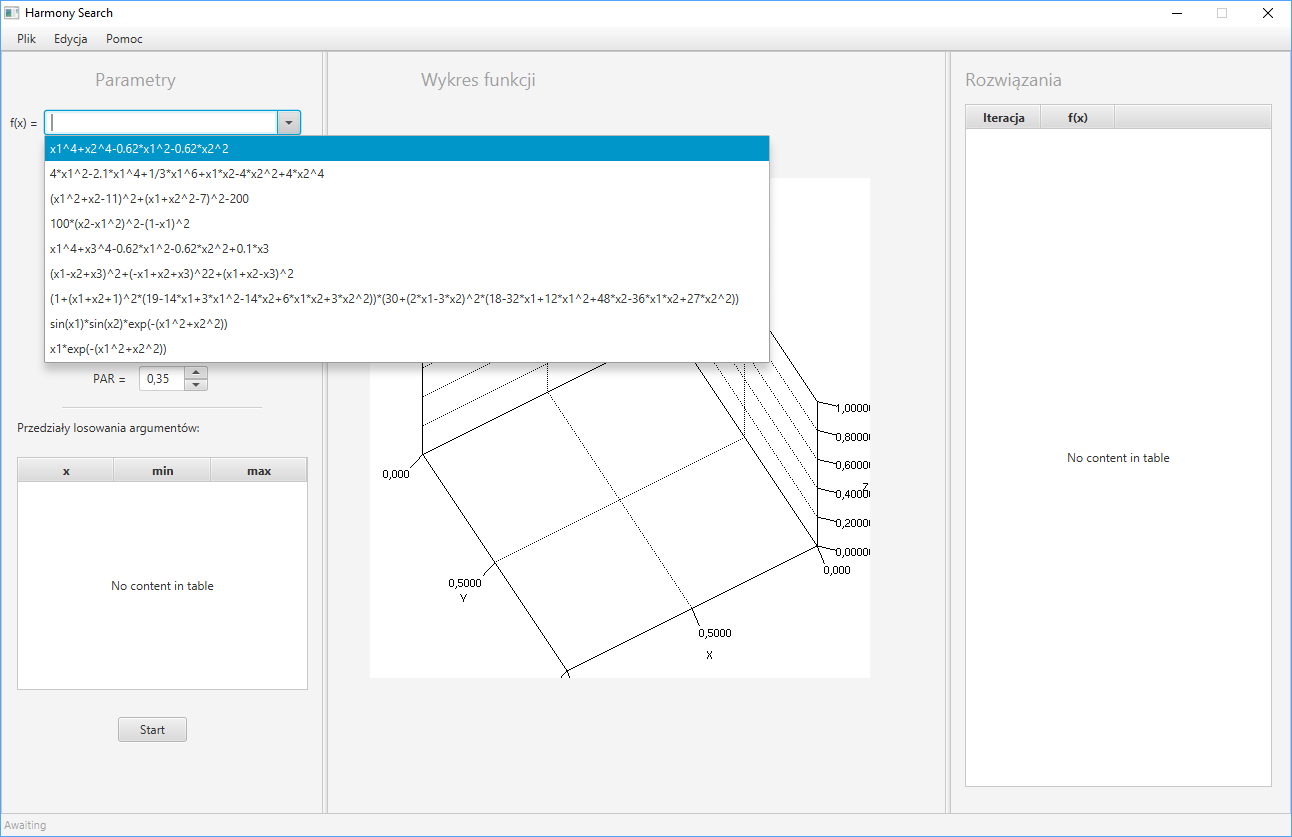
\includegraphics[width=\linewidth]{images/1.PNG} 
		\caption{Wpisywanie funkcji}
		\label{fig:1}
	\end{minipage} 
	\begin{minipage}[b]{.5\linewidth}
		\centering
		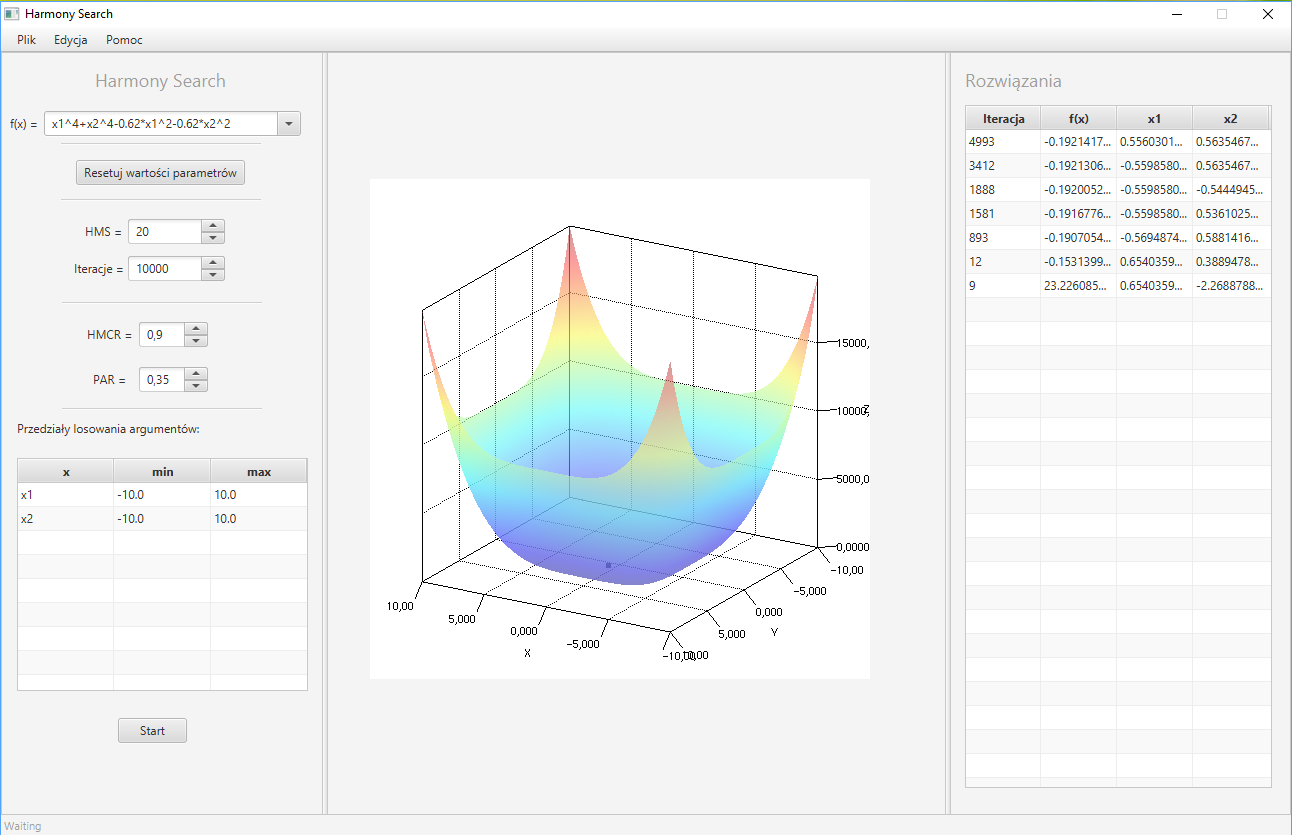
\includegraphics[width=\linewidth]{images/3.PNG} 
		\caption{Wykres z zaznaczonym rozwiązaniem}
		\label{fig:2}
	\end{minipage}
	\newline
	\newline
	\begin{minipage}[b]{1\linewidth}
		\centering
		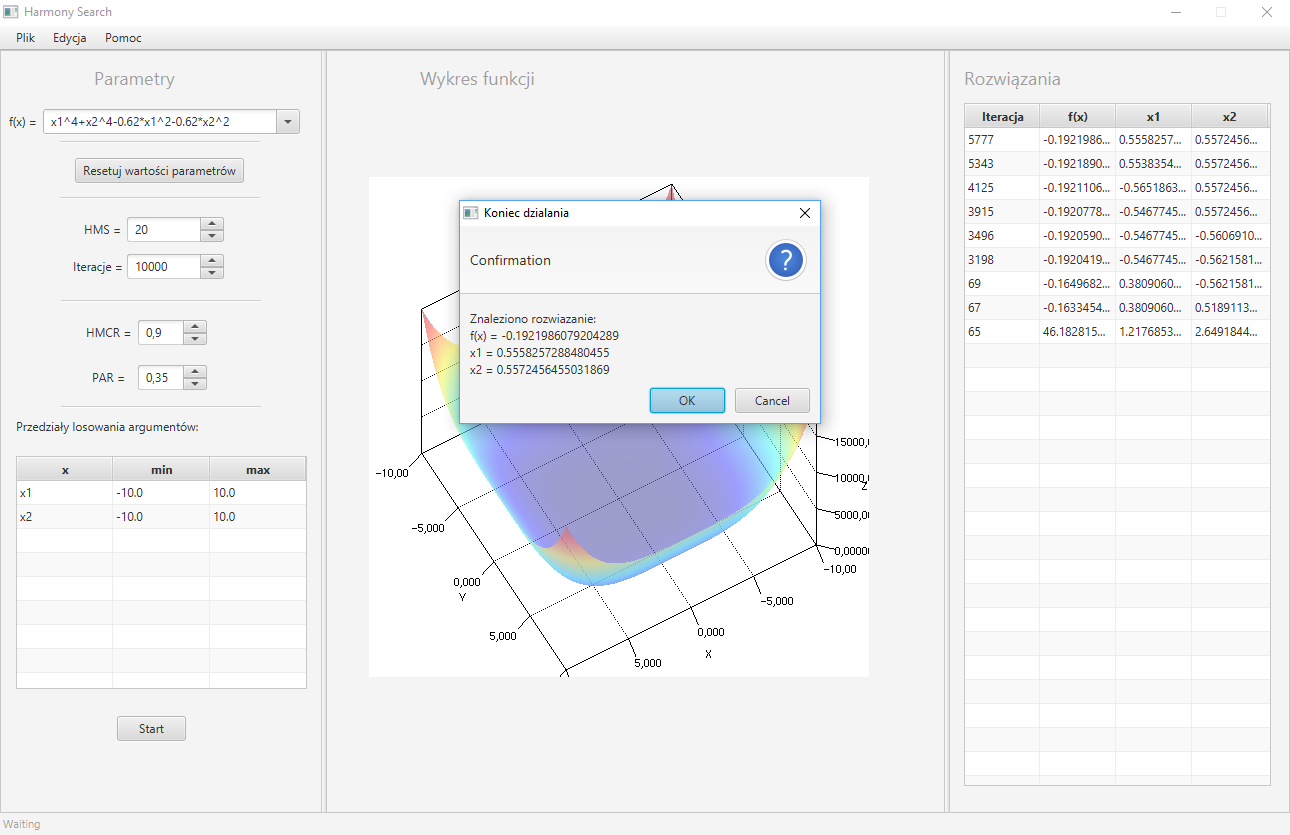
\includegraphics[width=.9\linewidth]{images/2.PNG} 
		\caption{Obliczone rozwiązanie wraz z komunikatem}
		\label{fig:3}
	\end{minipage}
\end{figure}

\pagebreak

\section{Przykłady rozwiązań oraz testy}
\label{sec:przyklady}
W tej części zostały przedstawione przykłady funkcji wraz z wynikami obliczonymi dzięki przedstawianemu programowi. 

\subsection{Funkcja czterech minimów}
\label{subsec:fcn4min}
Pierwsza zostanie przedstawiona funkcja posiadająca cztery minima lokalne. Wyraża się ona wzorem: $$f(x_{1},x_{2}) = x_{1}^{4}+x_{2}^{4}-0.62x_{1}^{2}-0.62x_{2}^{2}. $$  Rysunek \ref{fig:11} prezentuje trójwymiarowy wykres funkcji na przedziale $x_{1}, x_{2} \in <-1,1>$ wraz z zaznaczoną najmniejszą obliczoną wartością $f(x^*)=-0.19219, x^{*}(i) = [ \pm0.55672; \pm 0.55672], i = 1,...,4 $. 
\begin{figure}[htbp]
	\centering
		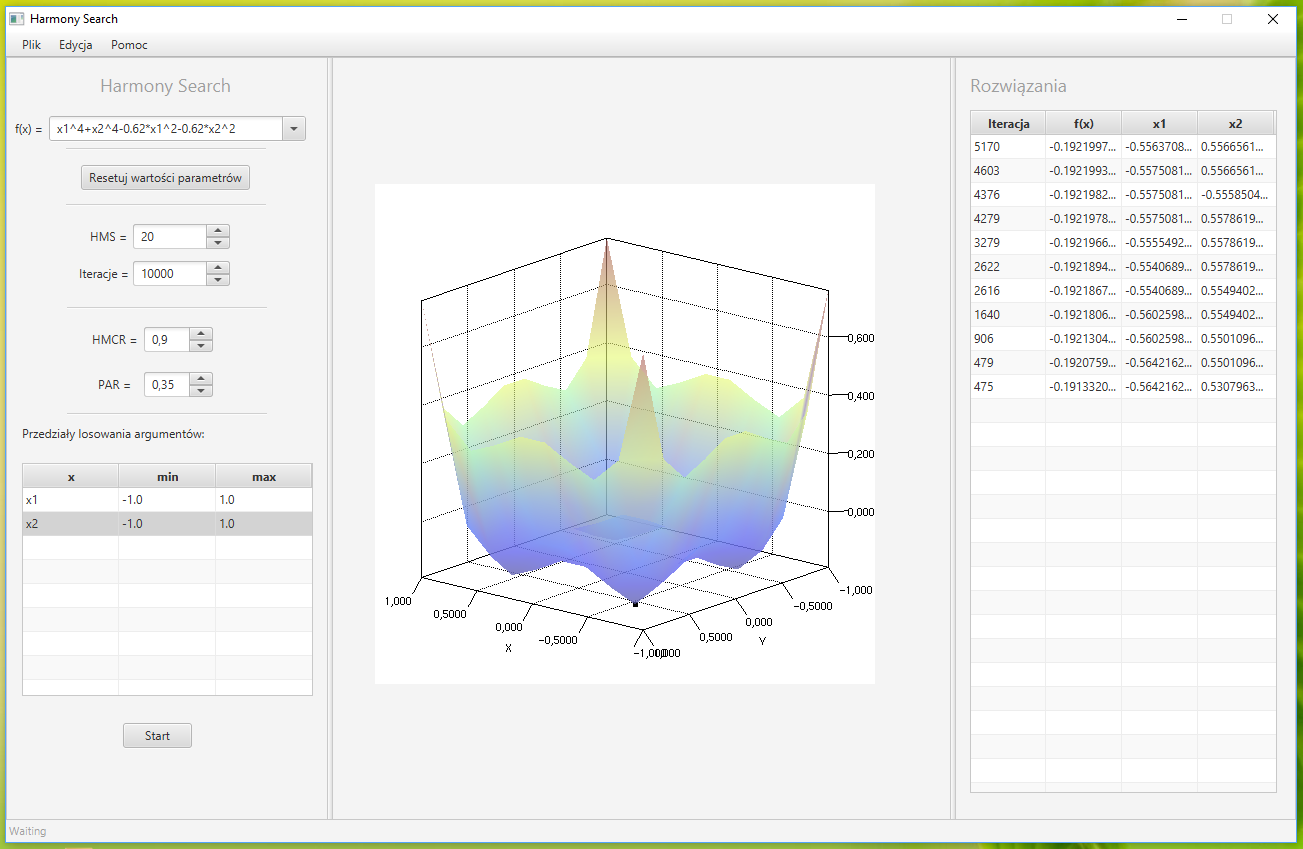
\includegraphics[width=.9\textwidth]{images/11.PNG}
		\caption{Wykres funkcji czterech minimów $x_{1}, x_{2} \in <-1,1>$}
		\label{fig:11}
\end{figure}

\subsubsection{Wyznaczenie wszystkich minimów}
\label{subsubsec:fcn4min2}
By wyznaczyć wszystkie minima funkcji należało zawęzić przedziały losowania argumentów w taki sposób, by w każdym przedziale było jedno minimum lokalne. Przypadki prezentowane na rysunkach \ref{fig:12}, kolejno pokazują każde obliczone minimum zależnie od podanego przedziału. Jak możemy dostrzec na wykresach algorytm znalazł poprawne rozwiązanie w każdym przedziale. Wartości minimum zaznaczone są na wykresach w~postaci czarnej kropki oraz wpisane są w najwyższy wiersz tabeli {\tt Rozwiązania} pokazanej po prawej stronie. 
\begin{figure}[htbp]
	\begin{minipage}[b]{1\textwidth}
		\centering
		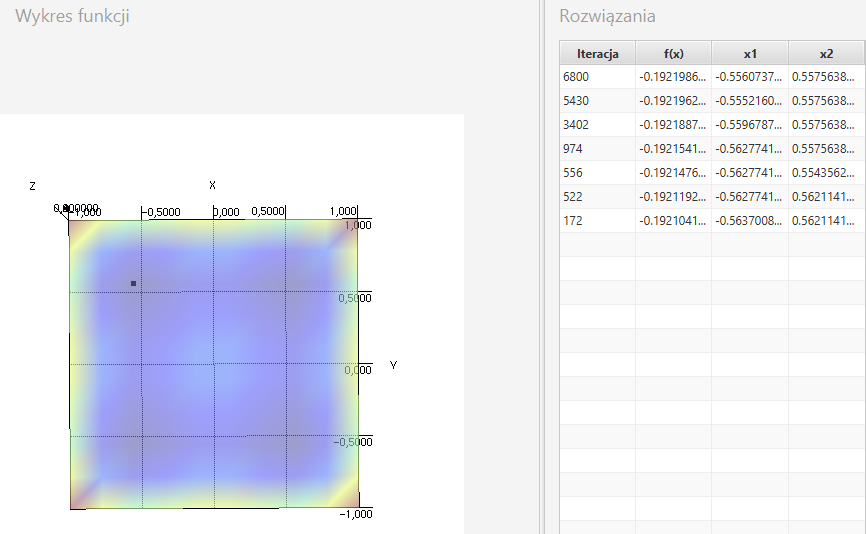
\includegraphics[width=\linewidth]{images/16e.PNG}
		\caption{Funkcja czterech minimów: $x_{1}\in<-1,0>,  x_{2}\in<0,1>$}
	\end{minipage}
	\begin{minipage}[b]{1\textwidth}
		\centering
		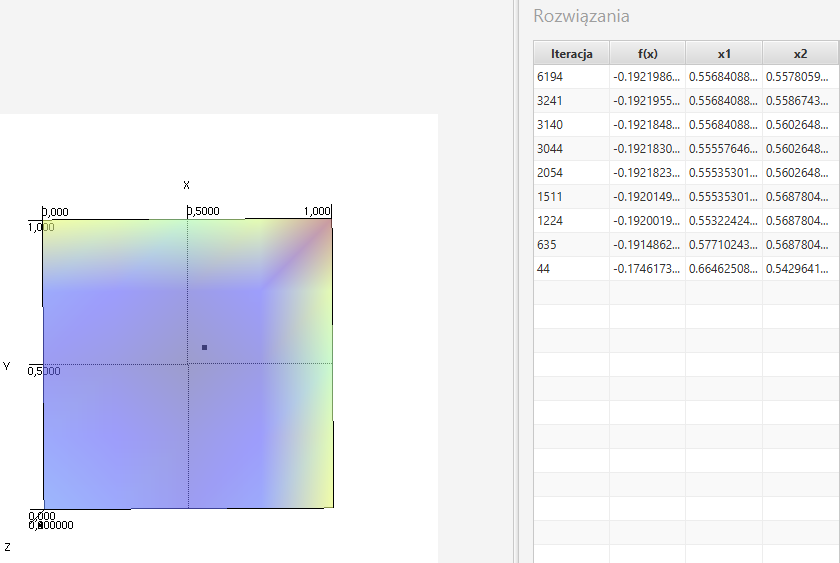
\includegraphics[width=\linewidth]{images/12e.PNG}
		\caption{Funkcja czterech minimów: $x_{1}\in<0,1>,  x_{2}\in<0,1>$}
	\end{minipage} 
\end{figure}
\begin{figure}[htbp]
	\begin{minipage}[b]{1\textwidth}
		\centering
		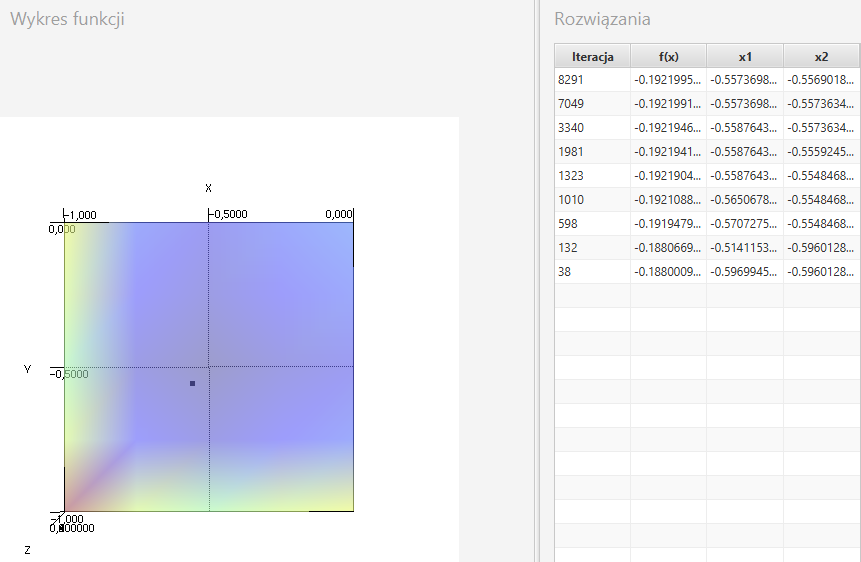
\includegraphics[width=\linewidth]{images/14e.PNG}
		\caption{Funkcja czterech minimów: $x_{1}\in<-1,0>,  x_{2}\in<-1,0>$}
	\end{minipage}
	\begin{minipage}[b]{1\textwidth}
		\centering
		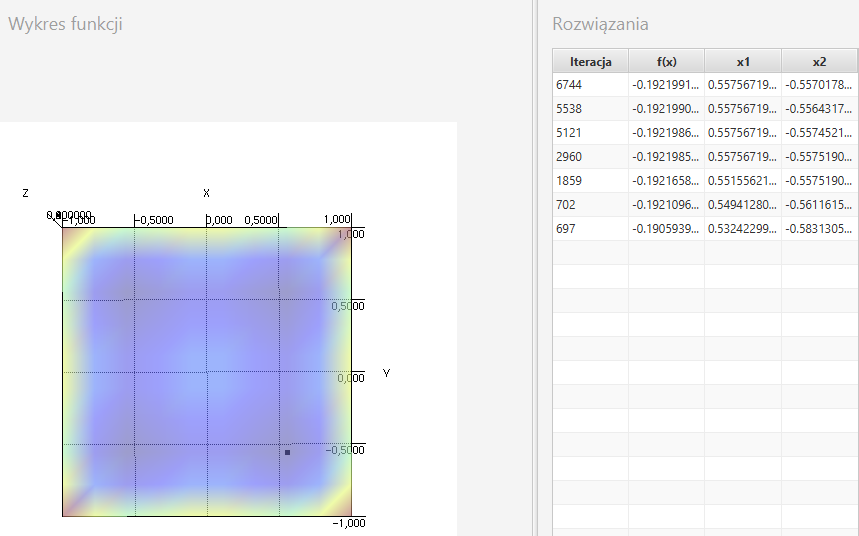
\includegraphics[width=\linewidth]{images/17e.PNG} 
		\caption{Funkcja czterech minimów: $x_{1}\in<0,1>,  x_{2}\in<-1,0>$}
	\end{minipage}
	\caption{Wykres funkcji czterech minimów dla różnych przedziałów}
	\label{fig:12}
\end{figure}

\pagebreak 

\subsection{Funkcja testowa Geema}
\label{subsec:gemm}
Kolejny przykład przedstawiał funkcję opisaną wzorem: $$f(x_{1},x_{2}) = x_{1}^{4}+x_{2}^{4}-0.62x_{1}^{2}-0.62x_{2}^{2}.$$ Jest to funkcja zwana szeciogarbnym wielbłądem: ma 6 minimów lokalnych, w tym 2 globalne: $f(x^*)=f(x^{**}=1.0316285, x^{*} = [ 0.08984, -0.71266], x^{**} = [- 0.08984, 0.71266]$. Początkowo zakres dla argumentów funkcji został przyjęty jako $x_{1},x_{2} \in <-0.5,1>$. Wykres funkcji wraz z rozwiązaniem zaprezentowany jest na rysunku \ref{fig:21}. 
\begin{figure}[htbp]
	\centering
	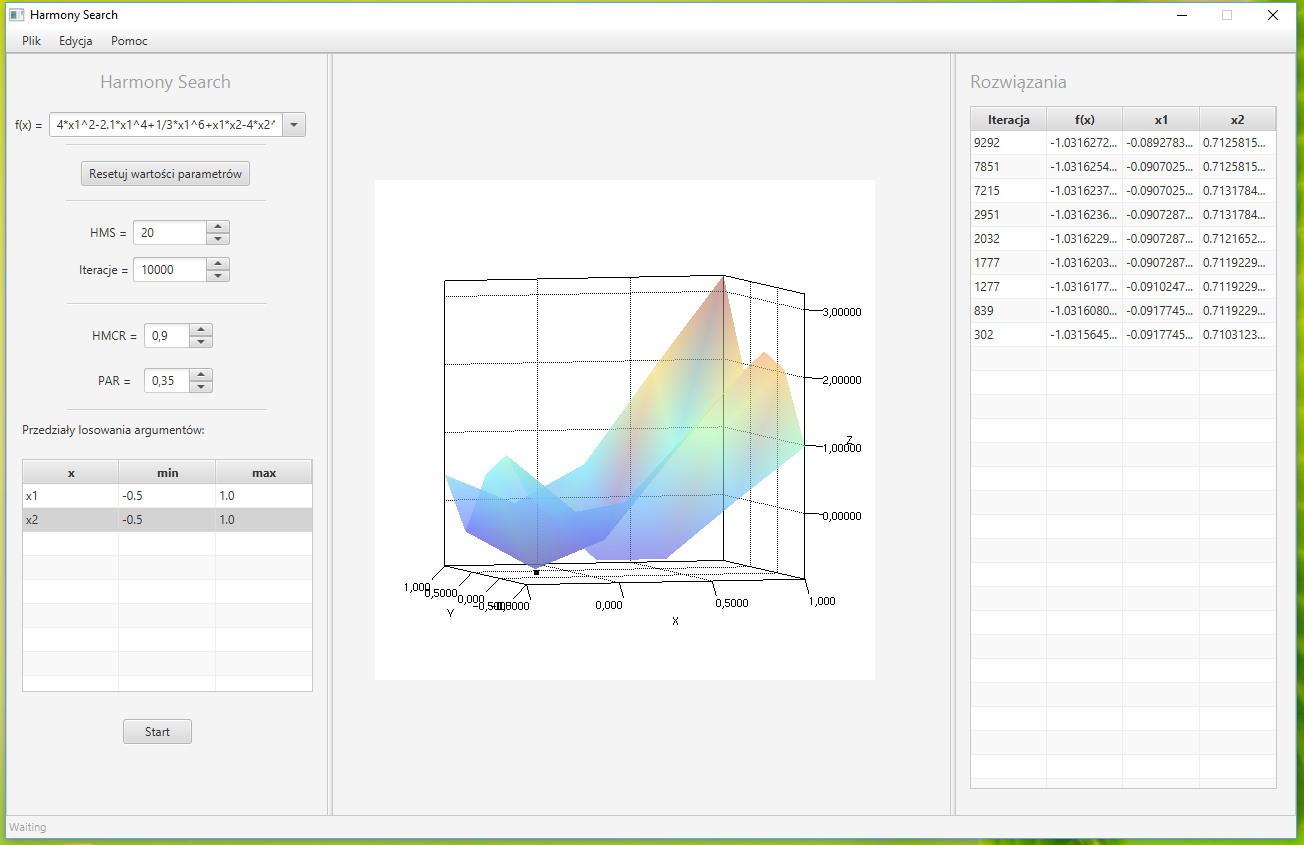
\includegraphics[width=1\textwidth]{images/21.PNG}
	\caption{Wykres funkcji Geema dla $x_{1}, x_{2} \in <-0.5,1>$}
	\label{fig:21}
\end{figure}

\subsubsection{Zmiana zakresu dla argumentów}
\label{subsubsec:gemm2}
Jak w poprzednim przykładzie tak i tutaj zmieniono zakres losowania argumentów na $x_{1}, x_{2} \in <-1,1>$. Zostały znalezione obydwa globalne minima.
\begin{figure}[htbp] 
	\begin{minipage}[b]{1\textwidth}
		\centering
		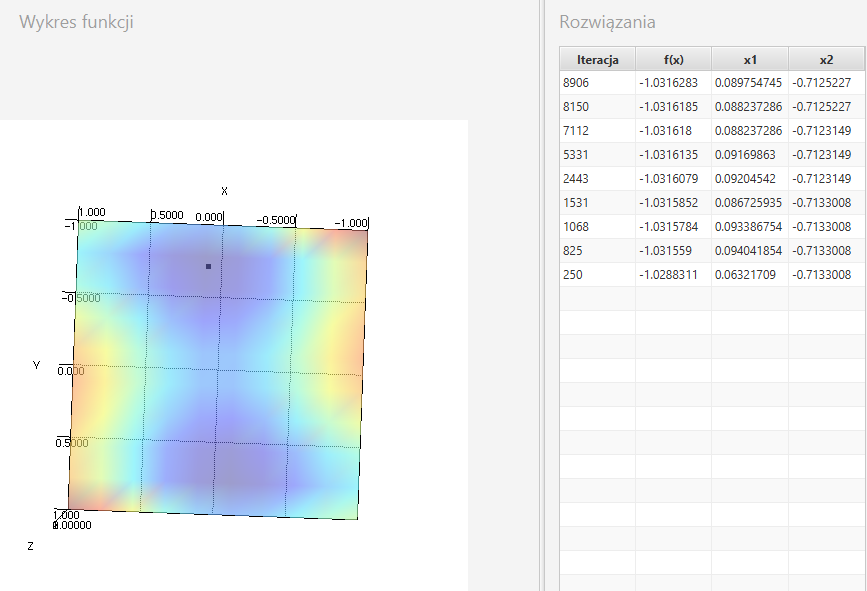
\includegraphics[width=\linewidth]{images/Geeme.PNG} 
	\end{minipage} 
	 \newline\newline
	\begin{minipage}[b]{1\textwidth}
		\centering
		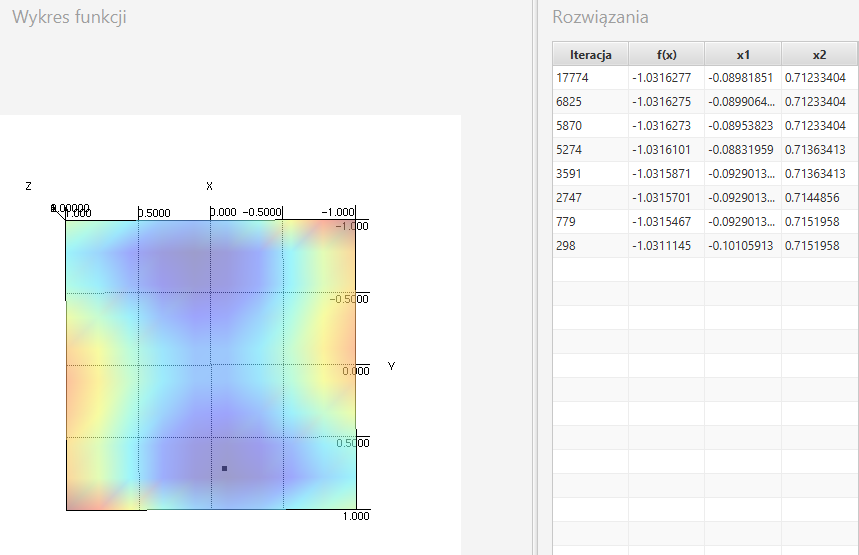
\includegraphics[width=\linewidth]{images/Geem2e.PNG} 
	\end{minipage}
	\caption{Wykresy funkcji Geema dla $x_{1}, x_{2} \in <-1,1>$}
	\label{fig:22}
\end{figure}

\pagebreak 

\subsection{Funkcja Rastrigina dla $n = 3$ }
\label{subsec:rastrigin}
Funkcja Rastrigina jest określona następująco: $$f(x) = \sum_{i=1}^{n} x_{i}^2-cos(18x_{i}), x_{i} \in <-1,1>.$$ Ma ona jedno globalne minimum $f(x^*) = -n, x^* = 0.$ W poniższym przypadku przyjęto $n=3$. Program odnajduje je bez większych problemów, chociaż im więcej iteracji, tym bardziej przybliża się do rzeczywistej wartości minimum.
\begin{figure}[htbp] 
	\begin{minipage}[b]{1\textwidth}
		\centering
		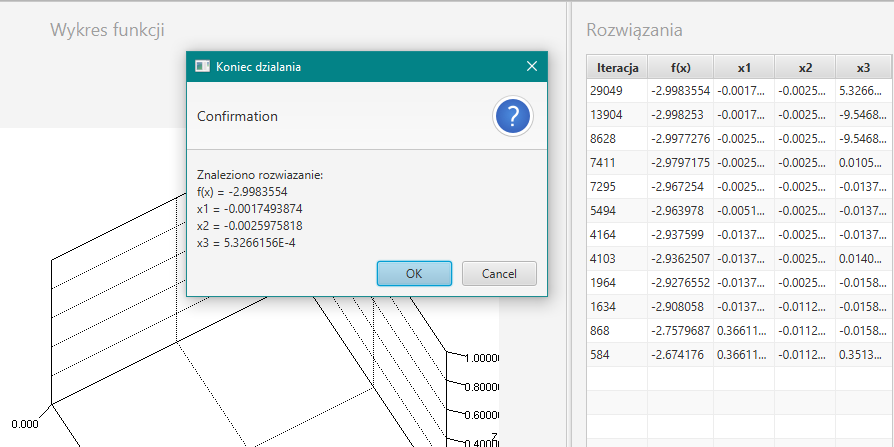
\includegraphics[width=\linewidth]{images/Rastrigine.PNG} 
	\end{minipage}
	\caption{Wykres funkcji Rastrigina i znalezione minimum globalne}
	\label{fig:23}
\end{figure}

\subsection{Funkcja Himmelblau}
\label{subsec:himmelblau}
Funkcja Himmelbalu również jak \ref{subsec:fcn4min} posiada cztery minima lokalne zlokalizowane po jednym w każdej ćwiartce na przedziale $x_{1,2} \in (-5,5)$. Funkcja posiada wzór: $$ f(x_{1},x_{2}) = (x_{1}^{2}+x_{2}-11)^{2}+(x_{1}+x_{2}^{2}-7)^{2}-200.$$ Dla pokazania, że funkcja wyszukuje rozwiązania z innego przedziału jak domyślny ograniczono się do przedziału z pierwszej ćwiartki $x_{1}, x_{2} \in (0,10)$. Na wykresie \ref{fig:31} zaprezentowany został wykres funkcji wraz z naniesionym najlepszym rozwiązaniem. 
\begin{figure}[htbp] 
	\begin{minipage}[b]{1\textwidth}
		\centering
		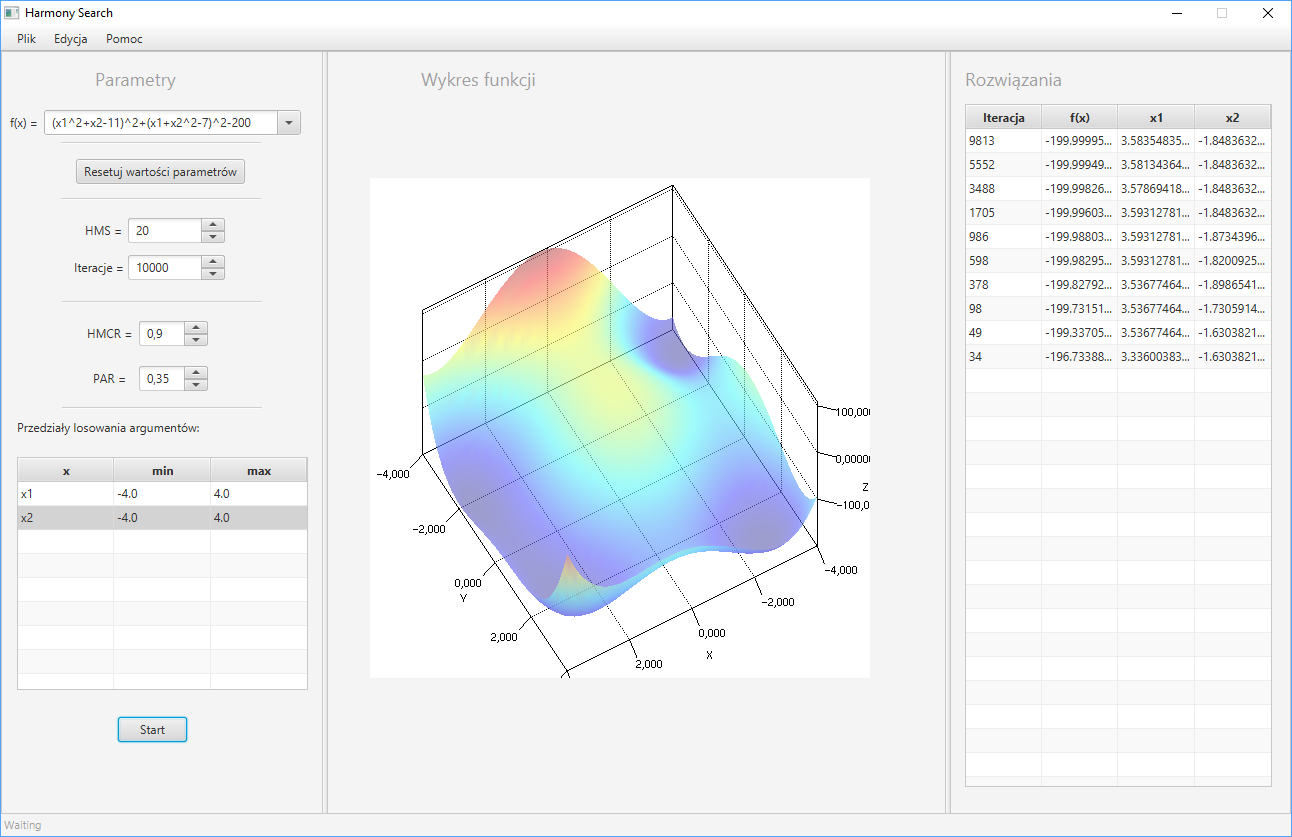
\includegraphics[width=\linewidth]{images/31.PNG} 
	\end{minipage} 
	\begin{minipage}[b]{1\textwidth}
		\centering
		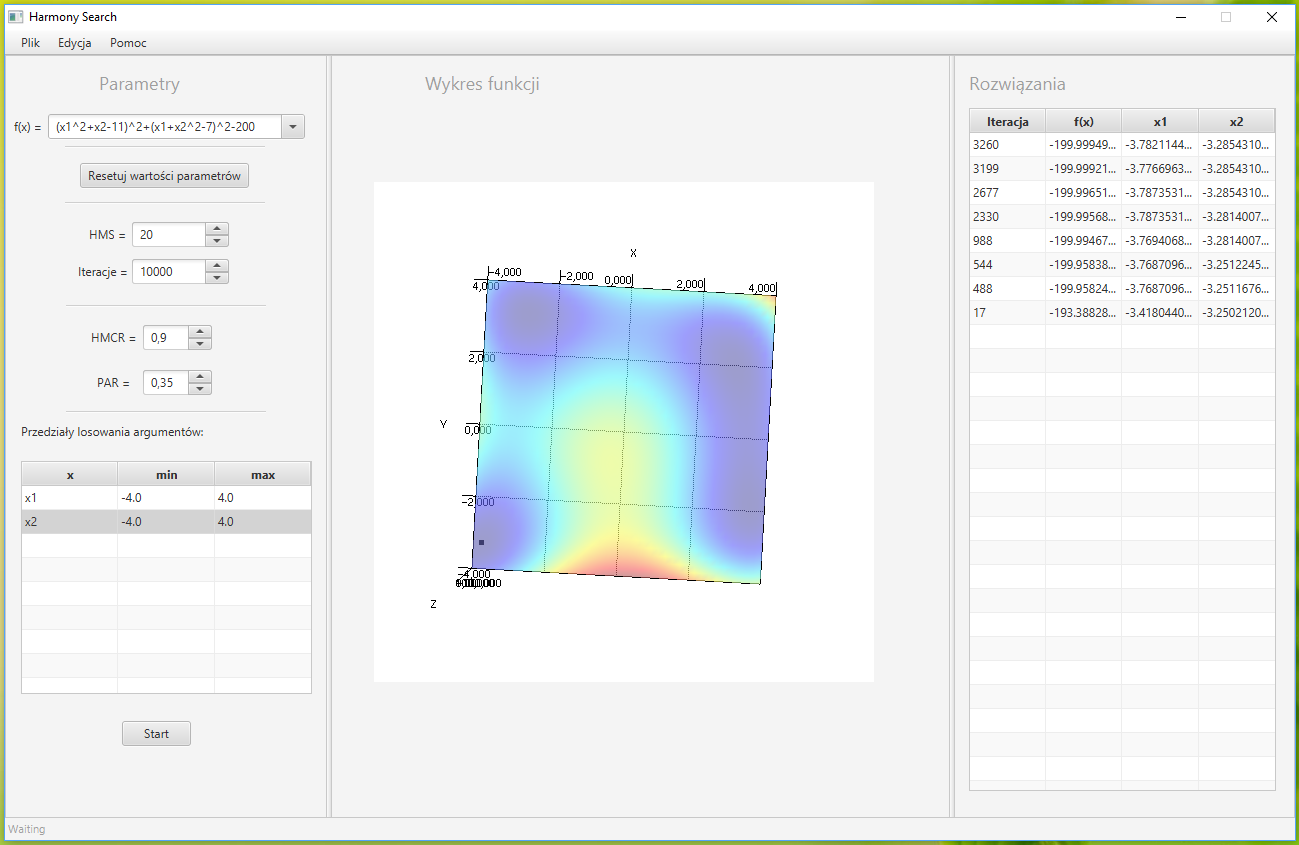
\includegraphics[width=\linewidth]{images/32.PNG} 
	\end{minipage}
	\caption{Wykresy funkcji Himmelblau dla $x_{1}, x_{2} \in <-4,4>$}
	\label{fig:31}
\end{figure}


\subsection{Funkcja Goldsteina-Price’a z czterema minimami lokalnymi}
\label{subsec:cenyzlota}
Funkcja Goldsteina-Price’a posiada kilka minimów lokalnych umiejscowionych blisko siebie. Opisuje ją wzór: $$f(x_{1},x_{2}) = [1+(x_{1}+x_{2}+1)^2(19-14x_{1}+3x_{1}^2-14x_{2}+6x_{1}x_{2}+3x_{2}^2)][30+(2x_{1}-3x_{2})^2(18-32x_{1}+12x_{1}^2+48x_{2}-36x_{1}x_{2}+27x_{2}^2)]$$ Odpowiednio manewrując parametrami algorytmu, program był w stanie obliczyć wszystkie 4 minima funkcji. Na wykresach \ref{fig:61} oraz \ref{fig:62} pokazano wyznaczone rozwiązania.
\begin{figure}[htbp] 
	\begin{minipage}[b]{1\textwidth}
		\centering
		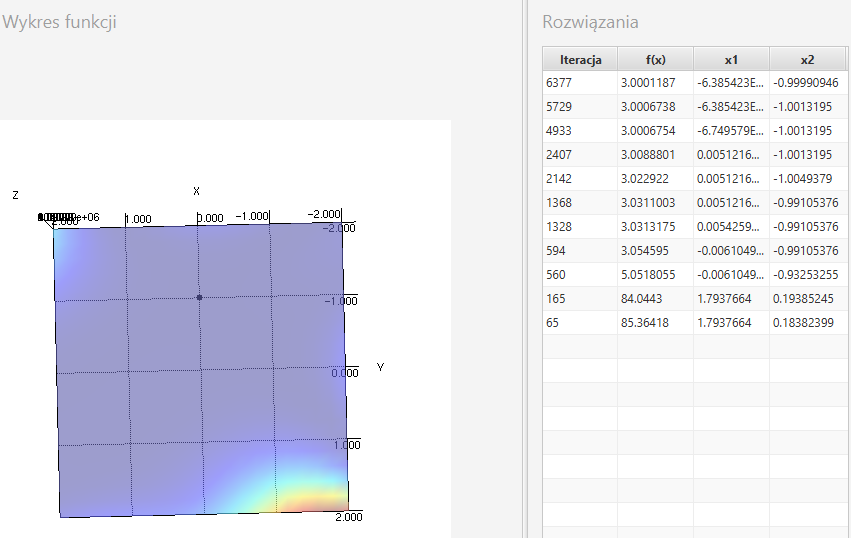
\includegraphics[width=\linewidth]{images/goldprice0.PNG}
		\caption{Wykres funkcji Goldsteina-Price’a z globalnym minimum: $x^*=[0.0; -1.0], f(x^*)=3.0$ }
	\end{minipage} 
	\begin{minipage}[b]{1\textwidth}
		\centering
		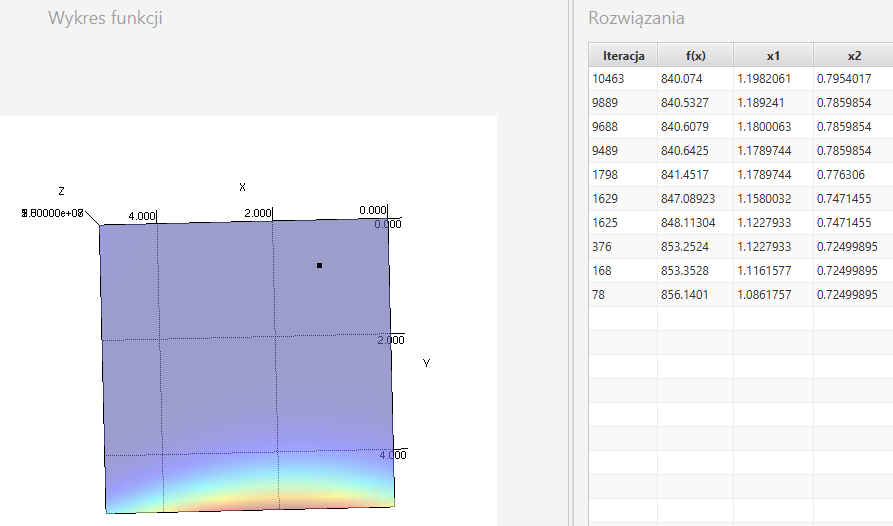
\includegraphics[width=\linewidth]{images/goldprice1.PNG} 
		\caption{Wykres funkcji Goldsteina-Price’a z lokalnym minimum: $x^*(1)=[1.2; 0.8], f[x^*(1)] = 840.0$ }
	\end{minipage}
	\caption{Wykresy funkcji Goldsteina-Price’a z lokalnymi minimami }
	\label{fig:61}
\end{figure}

\begin{figure}[htbp] 
	\begin{minipage}[b]{1\textwidth}
		\centering
		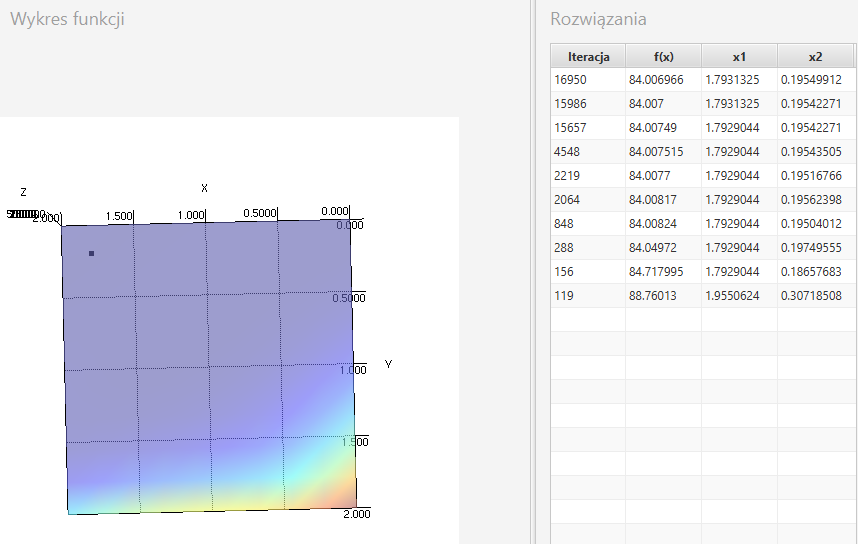
\includegraphics[width=\linewidth]{images/goldprice2.PNG}
		\caption{Wykres funkcji Goldsteina-Price’a z lokalnym minimum: $x^*(2)=[1.8; 0.2], f[x^*(2)]=84.0$ }
	\end{minipage} 
	\begin{minipage}[b]{1\textwidth}
		\centering
		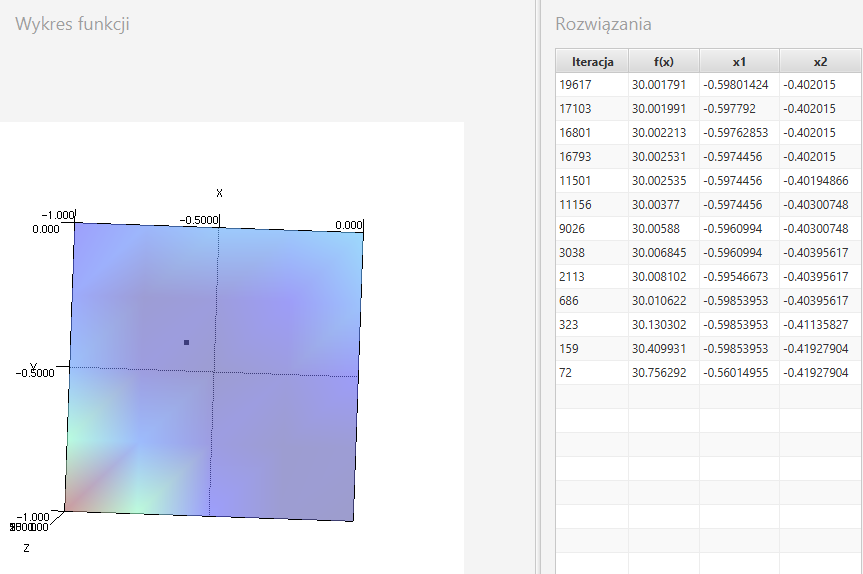
\includegraphics[width=\linewidth]{images/goldprice3.PNG}
		\caption{Wykres funkcji Goldsteina-Price’a z lokalnym minimum: $x^*(3)=[-0.6; -0.4], f[x^*(3)] = 30.0$ }
	\end{minipage}
	\caption{Wykresy funkcji Goldsteina-Price’a z lokalnymi minimami }
	\label{fig:62}
\end{figure}

\subsection{Dwuwymiarowa funkcja sinusoidalna}
\label{subsec:sin}
Dwuwymiarowa funkcja sinus posiada bardzo zróżnicowany przebieg oraz wiele równoważnych minimów lokalnych. Wzór funkcji przedstawiony jest równaniem $$f(x_{1},x_{2})=\sin{x_{1}}\sin{x_{2}}e^{-(x_{1}^2+x_{2}^2)}.$$ Rysunek \ref{fig:8} prezentuje wykres funkcji dla argumentów z przedziału $<-1,1>$.
\begin{figure}[htbp] 
	\begin{minipage}[b]{1\textwidth}
		\centering
		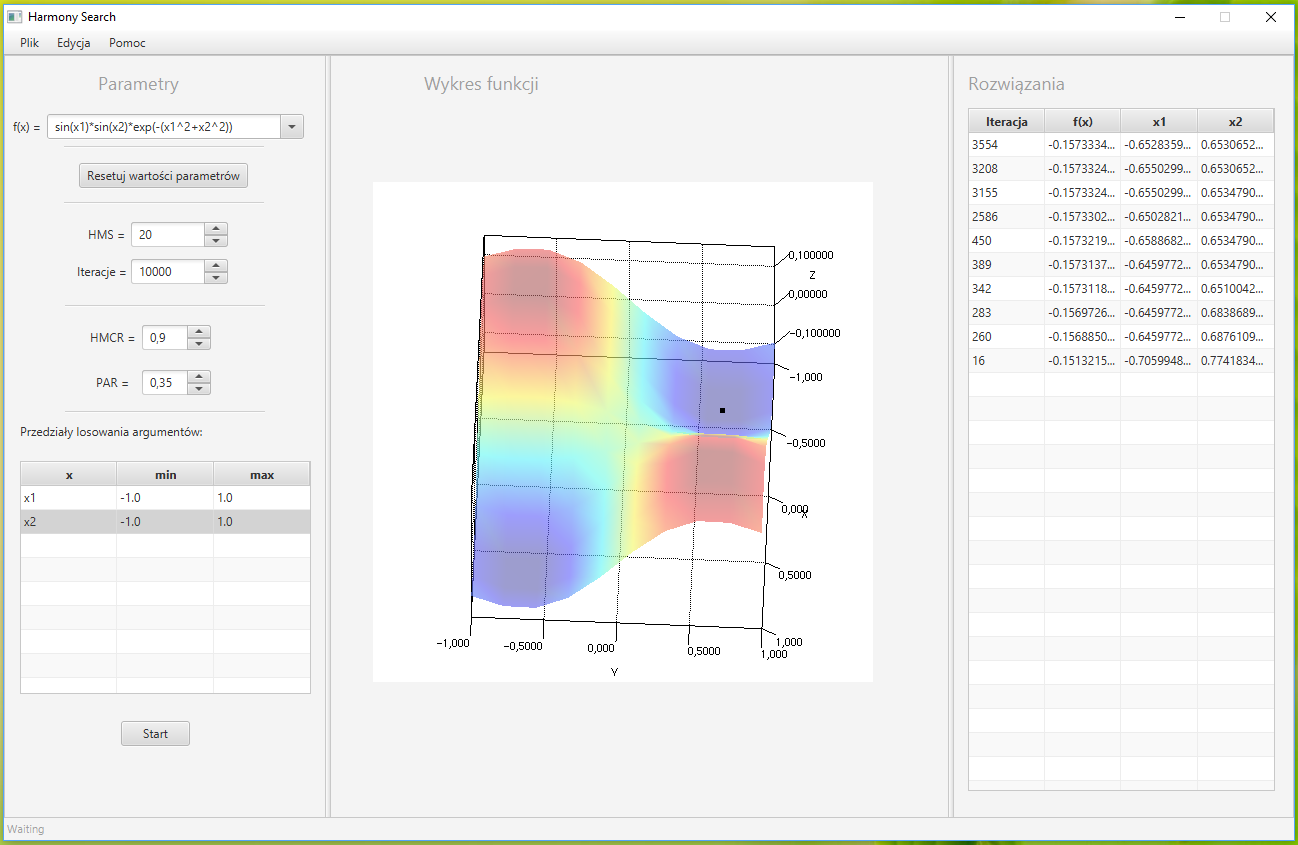
\includegraphics[width=\linewidth]{images/81.PNG}
	\end{minipage} 
	\begin{minipage}[b]{1\textwidth}
		\centering
		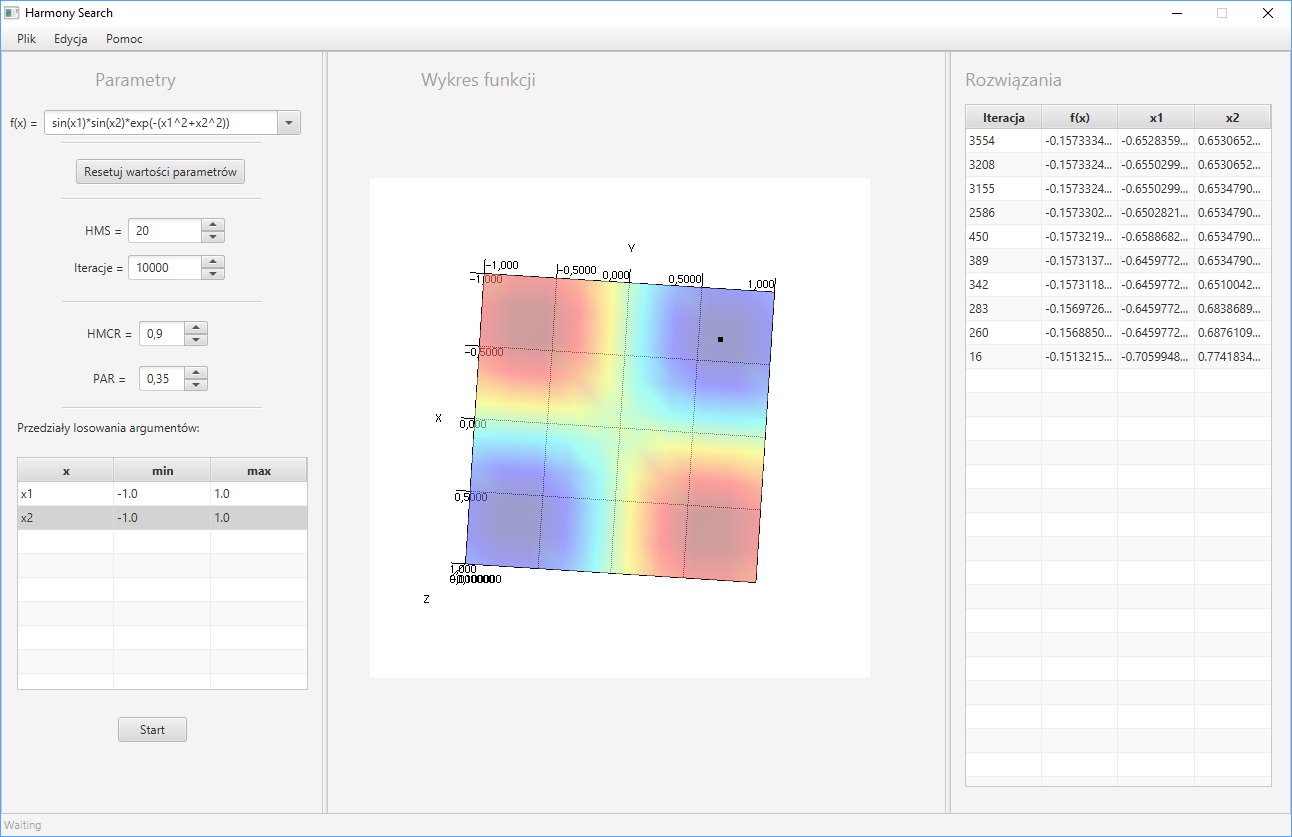
\includegraphics[width=\linewidth]{images/82.PNG} 
	\end{minipage}
	\caption{Wykres funkcji sinusoidalnej dla $x_{1}, x_{2} \in <-1,1>$}
	\label{fig:8}
\end{figure}

\subsection{Dwuwymiarowa funkcja sinusoidalna z eksponentą}
\label{subsec:sinexp}
Ostatnia przedstawiana funkcja ukazuje przypadek połączenia funkcji sinusa-cosinusa z eksponentą. Przypadek jest o tyle ciekawy, że większość wartości funkcji jest dla {\em $x_{1}, x_{2}$} jest do siebie zbliżona. Wzór funkcji przedstawiony jest jako: $$f(x)=x_{1}e^{-(x_{1}^{2}+x_{2}^2)}.$$ Rysunek \ref{fig:9} prezentuje działanie programu z obliczoną wartością minimalną. Program poprawnie wyliczył jej wartość, co potwierdza jego odporność na działanie funkcji, dla której większość argumentów jest stała. 
\begin{figure}[htbp] 
	\begin{minipage}[b]{1\textwidth}
		\centering
		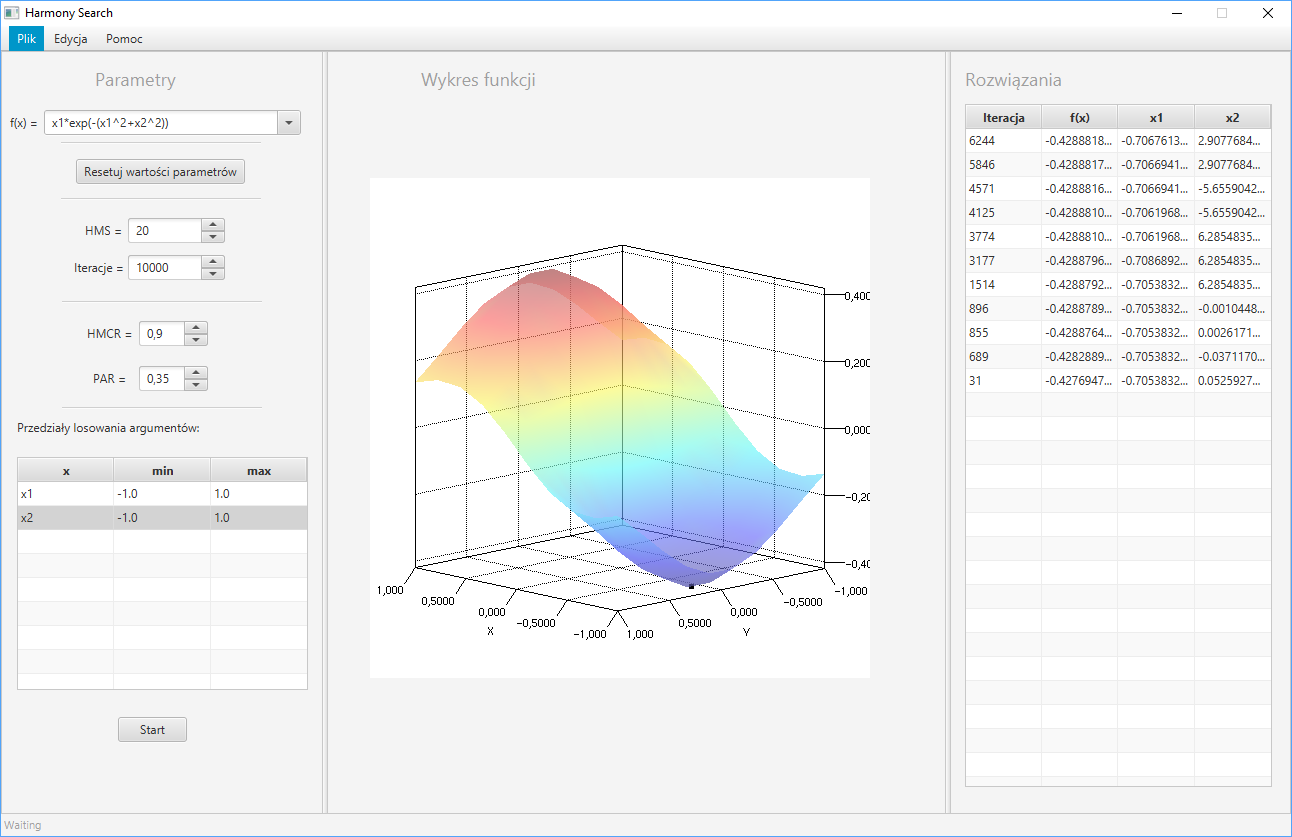
\includegraphics[width=\linewidth]{images/91.PNG}
	\end{minipage} 
	\begin{minipage}[b]{1\textwidth}
		\centering
		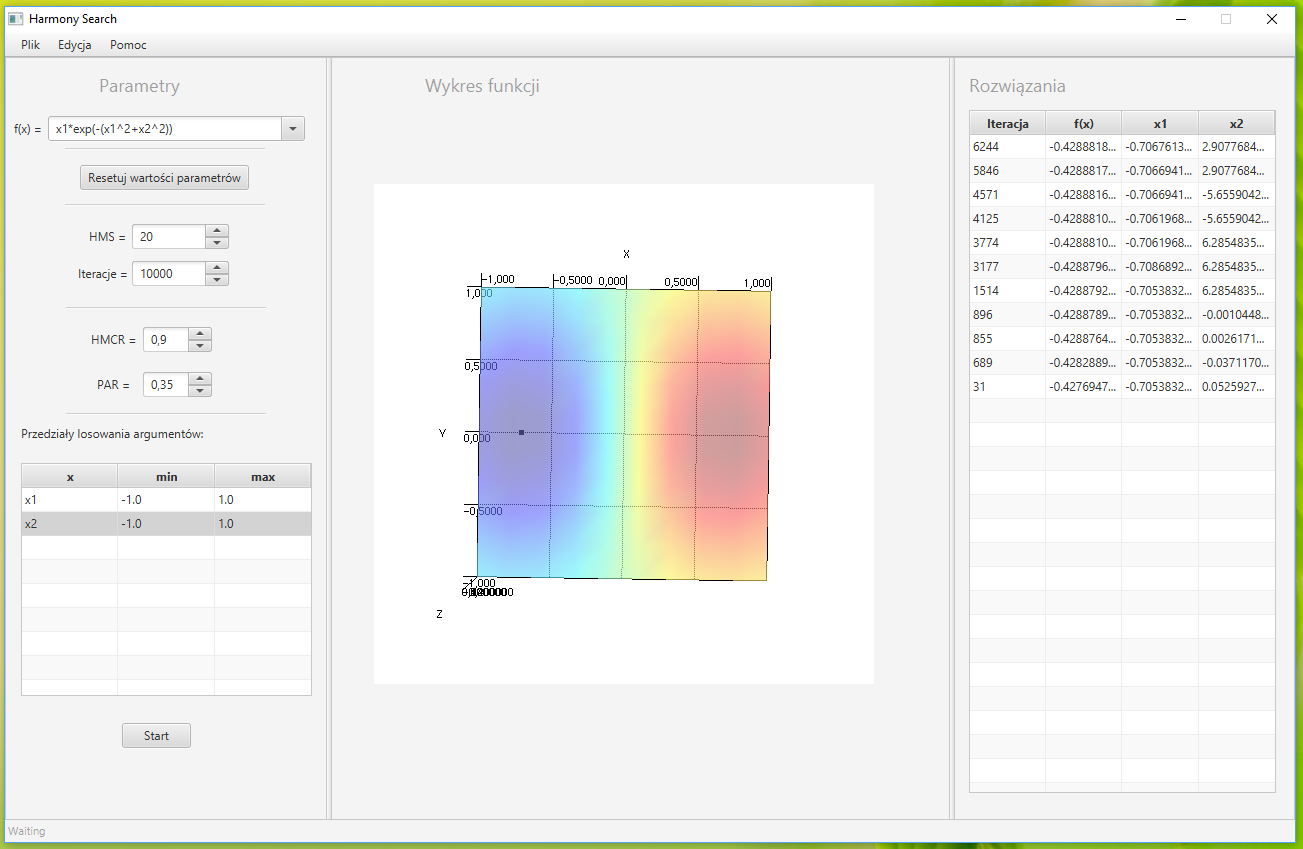
\includegraphics[width=\linewidth]{images/92.PNG} 
	\end{minipage}
	\caption{Wykres funkcji sinusoidalnej z eksponentą $x_{1}, x_{2} \in <-1,1>$}
	\label{fig:9}
\end{figure}

\subsection{Podsumowanie}
\label{subsec:podsumowanietestow}
Sprawdzając działanie programu dla różnych funkcji można stwierdzić, że poprawnie znajduje ich minima lokalne. Algorytm działa na tyle szybko, że dla użytkownika nie odczuwalny jest dyskomfort podczas użytkowania programu. Gdy funkcja posiada więcej niż jedno minimum, można znaleźć wszystkie z nich, odpowiednio kontrolując przedziały losowania argumentów lub liczbę iteracji. Można również sterować prawdopodobieństwami używanymi do generacji kolejnych rozwiązań, co może również pomóc w szybszym lub bardziej dokładnym znalezieniu szukanego minimum danej funkcji.

\pagebreak

\section{Wnioski końcowe}
\label{sec:wnioski}
Program obliczający minimum funkcji wielu zmiennych według algorytmu {\em Harmony Search} działa tak jak założono na początku. Spełniły się domniemania na temat szybkości działania algorytmu. Ponadto szybkość poprawiła się, gdy zamiast zwykłej tablicy dla {\tt HM} przyjęto {\tt SortedSet}. Program najdokładniej przybliży rozwiązanie, gdy zakres wartości {\em x} będzie jak najbliższy minimum funkcji. Dodatkowo, gdy ogranicznymy ilość iteracji, program zakończy szybciej swoje działanie, lecz kosztem znalezenia gorszego rozwiązania. Gdy wymagane jest obliczenie każdego z~minimum funkcji możemy je znaleźć i obliczyć jego wartość, o ile znamy przedział, w którym jest ono umiejscowione. Poprzez odpowiednie ustawienie parametrów algorymu i przedziałów losowania argumentów, jesteśmy w stanie wskazać kierunek poszukiwań lokalnych optimów funkcji.

Sam algorytm Harmony Search zyskuje coraz większą popularność w praktycznych zastosowaniach \cite{bib:geempdf}. Używa się do znajdywania rozwiązań problemów VRP ({\em ang. vehicle routing problem}, przykładowo szukanie optymalnej trasy szkolnych autobusów), projektowaniu sieci wodociągowych, systemów zapór wodnych czy pompy ciepła w satelitach. Zastosowanie znajduje także w innych dziedzinach: przewidywaniu struktury RNA, obróbce medycznych obrazów i onkologii, robotyce, śledzeniu wizualnym i wielu innych. Bardzo często daje lepsze rezultaty przy mniejszych błędach niż stosowane wcześniej metody, nie wymaga zadnych informacji o gradiencie funkcji, a także możliwe jest stosowanie do problemów dyskretnych. Wadą jest natomiast konieczność określenia parametrów działania, typowych dla algorytmów metaheurystycznych.

\newpage
\addcontentsline{toc}{section}{Literatura}
\bibliography{bibliografia}
\bibliographystyle{unsrt}
\end{document}

